\chapter{Spectrum sensing}

Spectrum sensing is the main task in the entire operation of cognitive
radio. Spectrum sensing is defined as the finding of spectrum holes in 
the local neighborhood of the cognitive radio receiver. Spectrum holes are the
underutilized (in part or in full) subbands of spectrum at a particular time
in a specific location. Moreover for cognitive radio to fulfil its potential
in solving the problem of spectrum underutilization, the spectrum sensing 
method used should be reliable and computationally feasible in real-time 
\cite{haykin09}.

There are many spectrum sensing techniques available. Three important ones of
them are as follows:
\begin{itemize}
    \item Energy detection
    \item Matched filter detection
    \item Cyclostationarity detection
\end{itemize}

\section{Energy detection}

Conventional energy detector is made up of a low pass filter, an A/D 
converter, a square law detector and an integrator (Figure 
\ref{energyDetection}a). This implementation is not flexible enough, 
especially in the case of narrowband signals and sinewaves. Also, this 
requires a pre-filter matched to the bandwidth $B$ of the signal to be scanned
\cite{cabric06}.

So, an alternative implementation is generally used where we find the squared 
magnitude of the FFT using the Average Periodogram method (Figure 
\ref{energyDetection}b). In this architecture, we can alter the bandwidth of
frequencies scanned just by taking
the required number of FFT bins. 

Spectrum sensing can be viewed as a binary hypothesis-testing problem 
\cite{zhang09}:
\begin{itemize}[noitemsep,topsep=0pt,parsep=0pt,partopsep=0pt]
    \item $H_0$: primary user is absent
    \item $H_1$: primary user is present
\end{itemize}
The detection is basically to decide between the following two hypotheses,
\begin{align}
    H_0 : \qquad x(t) &= n(t),  \nonumber \\
    H_1 : \qquad x(t) &= h(t)s(t) + n(t),  \nonumber
\end{align}
where $x(t)$ is the received signal, $s(t)$ is the primary user signal, $h(t)$
is the complex channel gain and $n(t)$ is the additive white gaussian noise
(AWGN) with zero mean and variance $\sigma_n^2$. Generally $h(t)$ is assumed
to be constant $h_0$ for the detection period. A statistics $Y$ is computed by
taking energy samples over a time $T$ in a bandwidth $B$ and compared with a 
predefined threshold $\gamma$ for making the decision.

Energy detection is one of the simplest methods of spectrum sensing. It is the 
optimal detection method for unknown signals. Moreover, it is widely used 
because its computationally less resource-intensive.

\begin{figure}
    \centering
    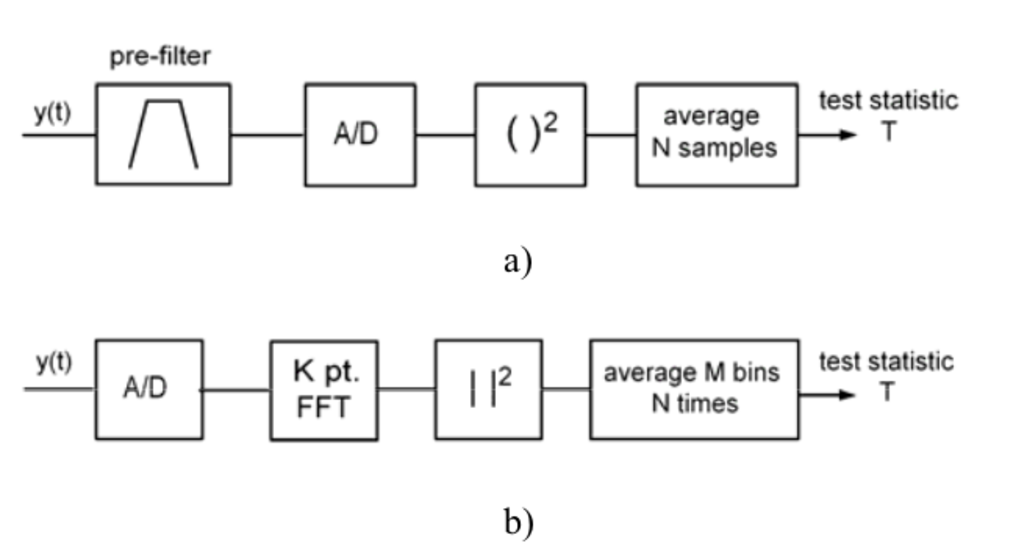
\includegraphics[width=0.7\textwidth]{../images/energyDetection}
    \caption[Energy Detection block diagram]{(a) Implementation using analog 
    filter and square law device \\
    (b) Implementation using periodogram. \\
    Source: {\cite{cabric06}}.}
    \label{energyDetection}
\end{figure}

But this method is not without problems. It is always to difficult to 
determine a threshold that will work for all situations. This method cannot
say whether an interfering signal is from a primary user or a secondary user.
Low SNR (signal to noise ratio) signals cannot be detected easily.

The frequency resolution can be improved by increasing N, the number of FFT 
points, but then this requires more samples and thereby takes more time.

\section{Matched filter detection}
A matched filter is a linear filter to maximize the output SNR of a received 
signal. It is the optimum filter to detect signals that are known a priori 
\cite{wikiMF}.


In matched filtering, the received signal is first band pass filtered and then
convolved with the impulse response. The impulse response $h$ here is the 
reference signal itself \cite{bhatta11}. Matched filtering is so called 
because the impulse response is matched to the reference signal.
\begin{equation*}
    Y[n] = \sum_{-\infty}^{\infty} h[n-k]x[k]
\end{equation*}

Here, $x[k]$ is the received or unknown signal with additive noise.
The goal of matched filtering is to enhance the component of reference signal
in the received signal and to suppress the noise. This works best when the 
additive noise is completely orthogonal to the reference signal or when the
noise is completely Gaussian. In practice though, the noise doesn't turn out 
to be purely Gaussian.
 
Matched filtering requires only $O$(1/SNR) samples to meet a given $P_d$, 
probability of detection requirement. Thus it requires less detection time.

But, matched filtering requires us to have a priori information about the 
received signal. This technique requires demodulating the received signal. For
demodulation, we require information like bandwidth, operating frequency, 
modulation type, pulse shaping, packet format, etc. Demodulating the received
signal correctly also requires timing synchronization, carrier 
synchronization, etc. It might still be possible to achive this because the
received data carry preambles, synchronization data, etc.

This method requires a specific type of receiver for every primary user.
Implementing this method on a receiver will increase the complexity and the 
power consumption greatly.

\begin{figure}
\centering
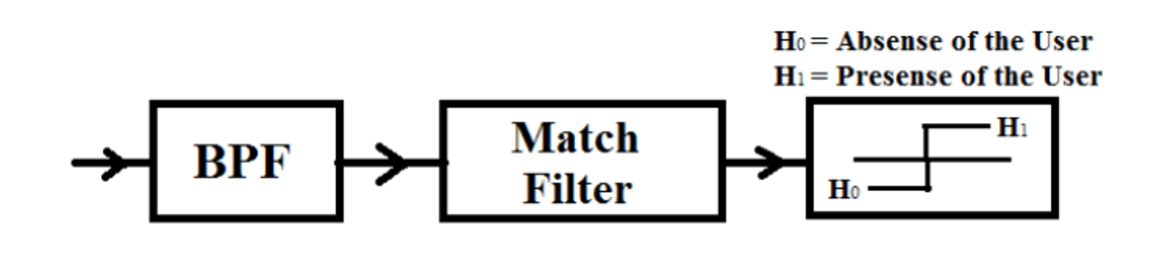
\includegraphics[width=0.8\textwidth]{../images/matchedFilter}
\caption[Matched filter]{Block diagram of Matched filter implementation.}
\label{matchedFilter}
\end{figure}

\section{Cyclostationarity detection}

To identify signals in the presence of noise and other signals, 
cyclostationarity detection uses the periodic properties of the signal. 
Sinusoidal waves, hopping sequences, cyclic prefixes, etc. of primary signals
carry periodic properties in them. These cyclostationary signals manifest 
spectral correlation and other periodic statistics while stationary noise and
interference do not.

These periodic properties are intentionally put in these signals to help the
receivers do timing synchronization, phase synchronization,
direction of arrival estimation \cite{kranthi13}, etc. These periodic 
properties help in identifying some random signal with particular modulation
types even in the midst of noise and interference from other signals.

In low SNR regions, cyclostationarity detection performs better than energy 
detection in identifying or detecting signals. Cyclostationarity detection is
very resistant to noise and other interferences. Although it requires some
a priori information, cyclostationarity can distinguish some Cognitive Radio
signals from primary signals.

The cons of cyclostationarity detection are that it is quite complicated 
mathematically, more computationally involved and requires longer observation
time.

We can detect a signal, given we know its cyclic frequency, by finding that
frequency in the SCD (Spectral Correlation Density) function calculated for 
the received signal. The SCD is also known as CS (Cyclic Spectrum) and SCF 
(Spectral Correlation Function).The SCD is given by \cite{deepa10}:
\begin{equation*}
    S_{x}^{\alpha}(f) = \int_{-\infty}^{\infty}R_{x}^{\alpha}(\tau)e^{-i2\pi 
    f\tau}d\tau
\end{equation*}
where the cyclic autocorrelation function $R_{x}^{\alpha}(\tau)$ is defined as
\cite{gardner91}
\begin{equation*}
    R_{x}^{\alpha}(\tau) {\buildrel\triangle\over =} \lim_{T\rightarrow\infty}
    \int_{-T/2}^{T/2}x(t+\tau/2)x^{\ast}(t-\tau/2)e^{-{i2\pi\alpha t}}dt
\end{equation*}
where $x(t)$ is the received signal and $\alpha$ is the 
\emph{cyclic frequency}.

\begin{figure}
\centering
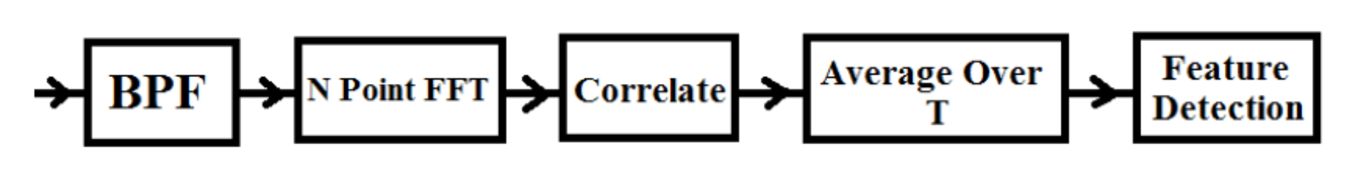
\includegraphics[width=0.7\textwidth]{../images/csd}
\caption[Cyclostationary Detection implementation]{Block diagram 
of Cyclostationary Detection implementation.}
\label{csd}
\end{figure}

We can also get the SCD function by considering a zero mean signal $x(t)$
whose time varying autocorrelation function $R_x(t,\tau)$ defined as
\cite{prithvi11}
\begin{equation*}
    R_{x}(t,\tau) = E\{x(t)x^{\ast}(t+\tau)\}
\end{equation*}
is periodic in time $t$ and can be represented as a Fourier series
\begin{equation*}
    R_{x}(t,\tau) = \sum_{\alpha}R_{x}^{\alpha} (\tau)e^{i2\pi\alpha t} 
\end{equation*}
for which the cyclic autocorrelation function is defined as
\begin{equation*}
    R_{x}^{\alpha}(\tau) = \lim_{T\rightarrow\infty} {\frac{1}{T}}
    \int_{\frac{T}{2}}^{\frac{T}{2}}R_{x}(t,\tau)e^{-i2\pi\alpha t}dT
\end{equation*}
Again the Fourier transform of $R_{x}^{\alpha}(\tau)$ is the SCD defined as
\begin{equation*}
    S_{x}^{\alpha}(\tau)=\int_{-\infty}^{\infty}R_{x}^{\alpha}
    (\tau)e^{-i2\pi f\tau}d\tau
\end{equation*}
Cyclic Spectrum is a two-dimensional transform whereas Power Spectral Density
(PSD) is just one-dimensional. Cyclostationarity detection won't work without
a priori information. But if we have all the a priori information, then 
matched filtering turns out to be a much simpler and faster technique.

\section{Comparison of sensing techniques}

\begin{figure}
\centering
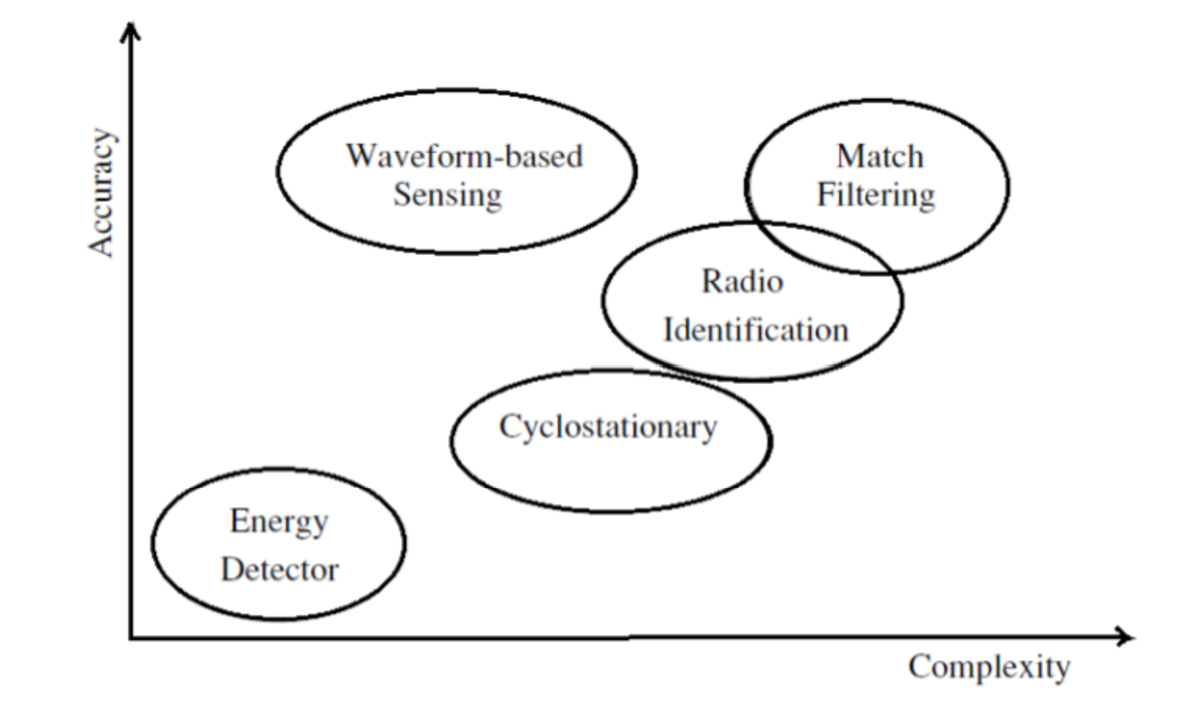
\includegraphics[width=0.77\textwidth]{../images/compareSensing}
\caption[Comparison of sensing methods]{Comparison of some spectrum sensing 
methods}
\label{compareSensing}
\end{figure}

Energy detection technique is the simplest method of all but it is also the 
most error prone. On the other hand, matched filtering is the most complex but 
it is very accurate. Cyclostationarity detection is more complicated than 
energy detection but it is more accurate. There is no ideal detection method.
There are always compromises and tradeoffs to be made. Figure 
\ref{compareSensing} shows a comparison of some spectrum sensing methods.

There are other methods of spectrum sensing that are more involved. For
example multitaper spectral estimation, wavelet based detection, waveform
based detection, etc.


\section{Implementation of energy detection technique}

In this section, we give a brief mathematical overview of the Average 
Periodogram Analysis method, that we have used in this project to calculate 
the energy in various operating frequencies. We also dwell on the wideband 
spectrum analyzer which happens to use the Average Periodogram Analysis 
method for doing its job.

\subsection{Average periodogram analysis}
This method applies the FFT (fast fourier transform) algorithm to the 
estimation of power spectra by sectioning the input time-domain data, finding
the modified periodogram for each section and then averaging them to get the
final spectral estimate. Since this method transforms the input data into 
smaller chunks, it requires less storage memory to implement this algorithm 
and also fewer computations. This is certainly an advantage and makes this 
method work faster. This method is also good for nonstationarity tests because
it has the potential to resolve the data in the time domain \cite{welch67}.

While computing the modified periodogram the data is smoothened using a window
because sharp transitions of data corrupt the modified periodograms. The 
window used in our project is the Blackman-Harris window.

Assume $X(n), n=0, ..., N-1$ is a sample from a stationary sequence. We take
segments, possibly overlapping, of length $L$ that are $D$ units apart from 
$X(n)$. Let $X_0(n)$ be the first such segment. Then $X_1(n) = X_0(n+D)$ and
$X_2(n) = X_1(n+D)$ and so on, where $n=0, ..., L-1$. We take $K$ segments
such that those $K$ segments almost use up all the data in $X(n)$ i.e.
$ (K-1)D + L = N$. Supposing $W(n), n=0, ..., L-1$ is the window, we calculate
the Discrete Fourier Transform (DFT) of each segment to get
\begin{equation*}
    A_k(m) = \frac{1}{L}\sum_{n=0}^{L-1}X_k(n)W(n)e^{-j2\pi nm/L} \qquad
    k = 0, ..., K-1
\end{equation*}

The $K$ modified periodograms are computed as 
\begin{equation*}
    I_k(f_m) = \frac{L}{U}\left|A_k(m)\right|^2 \qquad k = 0, ..., K-1
\end{equation*}
where
\begin{equation*}
    f_m = \frac{m}{L} \qquad m = 0, ..., L/2
\end{equation*}
and
\begin{equation*}
    U = \frac{1}{L}\sum_{n=0}^{L-1}W^2(n)
\end{equation*}
The spectral estimate is the average of these periodograms,
\begin{equation*}
    P(f_m) = \frac{1}{K}\sum_{k=0}^{K-1}I_k(f_m)
\end{equation*}

\subsection{Wideband Spectrum Analyzer}

GNURadio comes with a default spectrum analyzing program named 
``usrp\_spectrum\_sense.py''. This program can be used as a template for other
programs that involve spectrum analysis.

The output of this code is the squared magnitude of the FFT spectrum. For a 
typical FFT bin [i] the output is 
$Y[i] = re[X[i]]*re[X[i]] + im[X[i]]*im[X[i]]$. The power for a particular 
band can be calculated by summing these values for the correct number of bins
that cover that bandwidth. The energy in a particualar frequency corresponding
to a particular bin [i] is the square root of $Y[i]$. 

$N$ time samples of $x(t)$ sampled at a sampling frequency of $F_{s}$ are 
required to use $N$ point complex FFT $X(\omega)$ analysis. To reduce spectral
leakage, an appropriate window function like Blackman-Harris window is to be 
chosen  and applied to these time samples. The output of the FFT represents 
the spectrum content as follows:

\begin{itemize}
    \item The first value of the FFT output $(bin0 == X[0])$ corresponds to 
    the energy in the centre frequency.
    \item The first half of the FFT spectrum ($X[1]$ to $X[N/2-1]$) 
    corresponds to the positive baseband frequencies i.e. from the centre 
    frequency to $+F_{s}/2$.
    \item The second half ($X[N/2]$ to $X[N-1]$) corresponds to the negative 
    baseband frequencies, i.e. from $-F_{s}/2$ to the centre frequency.
\end{itemize}


For the purposes of our project, we used to collect N = 1024 samples using a 
radio tuner centered at the frequency of our interest, say 900 MHz. The number
of FFT points, N should be a power of 2 for the FFT algorithm to work fast, so
we set N = 1024 for our work. We set the sampling frequency to be 1 MHz 
because all we are required to do is scan GSM bands that are of 200 KHz each. 
The frequency resolution thus turns out to be: 1 MHz / 1024 = 976.56 KHz. The 
decimation factor is defined as the dsp rate divided by the sampling rate. The
dsp rate is the actual hardware sampling rate of the ADC in the USRP kit and 
was 100 MHz in our case. The UHD driver (driver software for the USRP kits)
requires the decimation factor to be an integer value. So we set our sampling 
rate to 1 MHz which made the decimation factor to be 100 MHz / 1 MHz = 100, an
integer value. For example if we set the sampling rate as 3 MHz then the 
USRP's driver would complain because the decimation factor 100 MHz / 1 MHz = 
33.33 turns out to be a non-integral value.

As has been said earlier, a GSM band is of 200 KHz. Hence, to calculate the 
energy in a particular GSM band of interest, we have to find the average of 
all the bin values which lie in the 200 KHz band centered at that frequency.


